\documentclass[hidelinks,12pt]{article}

\usepackage[italian]{babel}
\usepackage[a4paper]{geometry}
\usepackage{amsmath, tikz, hyperref, caption, subcaption}
\usepackage[capitalize, italian]{cleveref}
\usepackage[
   backend=biber,
   style=numeric,
 ]{biblatex}
\addbibresource{bib/db.bib}

% -- Font settings
\usepackage[math-style=ISO]{unicode-math}
\setmainfont{EB Garamond}%You should have installed the font
\setmathfont{Garamond-Math.otf}[StylisticSet={8,9}]
\setmathfont{Garamond-Math.otf}[range={scr,bfscr}]

\setlength{\parskip}{1.2ex}
\setlength{\parindent}{0em}
\clubpenalty = 100
\widowpenalty = 100

\title{STM32 GameBoy}
\date{\today}
\author{Marco Cutecchia, Edoardo Marangoni \\
\footnotesize \texttt{\{marco.cutecchia, edoardo.marangoni1\}@studenti.unimi.it} \\ }

\begin{document}
\maketitle

\section{Introduzione}
Il GameBoy è una console portatile rilasciata da Nintendo all'inizio degli anni
90 che diede inizio al grandissimo successo dei videogiochi tascabili.
La console vendette più di 118 milioni di unità nel mondo e divenne un fenomeno
culturale ricordato ancora oggi.

Lo scopo del progetto è quello di costruire un'imitazione del GameBoy in grado
di giocare tutti i videogiochi originali, ma con una serie di miglioramenti
grazie ai componenti hardware più moderni. Tra le modifiche al dispositivo
originale che abbiamo implementato troviamo il caricamento dei giochi tramite
microSD, invece che con cartucce, e l'utilizzo di uno schermo a colori e
retroilluminato, al contrario dell'originale schermo a scala di grigi che
diventava impossibile da vedere sotto scarsa luce.

\section{Hardware}
Le componenti hardware utilizzate sono tre: il microcontrollore
\texttt{STM32F411CEU6} (\cref{fig:weact_blackpill}), lo schermo \texttt{ILI9341}
(\cref{fig:ili9341}) e la PCB per la plancia di gioco
(\cref{fig:pcb}).

\subsection{Microcontrollore}
La componente centrale del progetto è il microcontrollore
\texttt{STM32F411CEU6}, prodotto da ST, montato sulla board \texttt{WeAct Black
	Pill V2.0}. Il microcontrollore monta un core \texttt{arm} Cortex-M4 con clock
massimo di $100$MHz. Questo microcontrollore offre $34$ pin GPIO che verranno
utilizzati per collegare il microcontrollore a schermo e pad; monta $512$KiB di
memoria flash e $128$KiB di SRAM, necessari per l'esecuzione del software
che abbiamo utilizzato.
\begin{figure}
	\begin{subfigure}[b]{0.45\textwidth}
		\begin{center}
			\begin{tikzpicture}[x=0.015cm, y=0.015cm, scale=0.5, transform shape]
					\draw  [color={rgb, 255:red, 0; green, 0; blue, 0 }  ,draw opacity=1 ][fill={rgb, 255:red, 255; green, 255; blue, 255 }  ,fill opacity=1 ] (480,140) -- (640,140) -- (640,960) -- (480,960) -- cycle ;
	\draw  [fill={rgb, 255:red, 255; green, 255; blue, 255 }  ,fill opacity=1 ] (440,150) -- (510,150) -- (510,190) -- (440,190) -- cycle ;
	\draw  [fill={rgb, 255:red, 255; green, 255; blue, 255 }  ,fill opacity=1 ] (440,190) -- (510,190) -- (510,230) -- (440,230) -- cycle ;
	\draw  [fill={rgb, 255:red, 255; green, 255; blue, 255 }  ,fill opacity=1 ] (440,230) -- (510,230) -- (510,270) -- (440,270) -- cycle ;
	\draw  [fill={rgb, 255:red, 255; green, 255; blue, 255 }  ,fill opacity=1 ] (440,270) -- (510,270) -- (510,310) -- (440,310) -- cycle ;
	\draw  [fill={rgb, 255:red, 255; green, 255; blue, 255 }  ,fill opacity=1 ] (440,310) -- (510,310) -- (510,350) -- (440,350) -- cycle ;
	\draw  [fill={rgb, 255:red, 255; green, 255; blue, 255 }  ,fill opacity=1 ] (440,350) -- (510,350) -- (510,390) -- (440,390) -- cycle ;
	\draw  [fill={rgb, 255:red, 255; green, 255; blue, 255 }  ,fill opacity=1 ] (440,390) -- (510,390) -- (510,430) -- (440,430) -- cycle ;
	\draw  [fill={rgb, 255:red, 255; green, 255; blue, 255 }  ,fill opacity=1 ] (440,430) -- (510,430) -- (510,470) -- (440,470) -- cycle ;
	\draw  [fill={rgb, 255:red, 255; green, 255; blue, 255 }  ,fill opacity=1 ] (440,470) -- (510,470) -- (510,510) -- (440,510) -- cycle ;
	\draw  [fill={rgb, 255:red, 255; green, 255; blue, 255 }  ,fill opacity=1 ] (440,510) -- (510,510) -- (510,550) -- (440,550) -- cycle ;
	\draw  [fill={rgb, 255:red, 255; green, 255; blue, 255 }  ,fill opacity=1 ] (440,550) -- (510,550) -- (510,590) -- (440,590) -- cycle ;
	\draw  [fill={rgb, 255:red, 255; green, 255; blue, 255 }  ,fill opacity=1 ] (440,630) -- (510,630) -- (510,670) -- (440,670) -- cycle ;
	\draw  [fill={rgb, 255:red, 255; green, 255; blue, 255 }  ,fill opacity=1 ] (440,670) -- (510,670) -- (510,710) -- (440,710) -- cycle ;
	\draw  [fill={rgb, 255:red, 255; green, 255; blue, 255 }  ,fill opacity=1 ] (440,710) -- (510,710) -- (510,750) -- (440,750) -- cycle ;
	\draw  [fill={rgb, 255:red, 255; green, 255; blue, 255 }  ,fill opacity=1 ] (440,750) -- (510,750) -- (510,790) -- (440,790) -- cycle ;
	\draw  [fill={rgb, 255:red, 255; green, 255; blue, 255 }  ,fill opacity=1 ] (440,790) -- (510,790) -- (510,830) -- (440,830) -- cycle ;
	\draw  [fill={rgb, 255:red, 255; green, 255; blue, 255 }  ,fill opacity=1 ] (440,830) -- (510,830) -- (510,870) -- (440,870) -- cycle ;
	\draw  [fill={rgb, 255:red, 255; green, 255; blue, 255 }  ,fill opacity=1 ] (440,870) -- (510,870) -- (510,910) -- (440,910) -- cycle ;
	\draw  [fill={rgb, 255:red, 255; green, 255; blue, 255 }  ,fill opacity=1 ] (440,910) -- (510,910) -- (510,950) -- (440,950) -- cycle ;
	\draw  [fill={rgb, 255:red, 255; green, 255; blue, 255 }  ,fill opacity=1 ] (610,150) -- (680,150) -- (680,190) -- (610,190) -- cycle ;
	\draw  [fill={rgb, 255:red, 255; green, 255; blue, 255 }  ,fill opacity=1 ] (610,190) -- (680,190) -- (680,230) -- (610,230) -- cycle ;
	\draw  [fill={rgb, 255:red, 255; green, 255; blue, 255 }  ,fill opacity=1 ] (610,230) -- (680,230) -- (680,270) -- (610,270) -- cycle ;
	\draw  [fill={rgb, 255:red, 255; green, 255; blue, 255 }  ,fill opacity=1 ] (610,270) -- (680,270) -- (680,310) -- (610,310) -- cycle ;
	\draw  [fill={rgb, 255:red, 255; green, 255; blue, 255 }  ,fill opacity=1 ] (610,310) -- (680,310) -- (680,350) -- (610,350) -- cycle ;
	\draw  [fill={rgb, 255:red, 255; green, 255; blue, 255 }  ,fill opacity=1 ] (610,350) -- (680,350) -- (680,390) -- (610,390) -- cycle ;
	\draw  [fill={rgb, 255:red, 255; green, 255; blue, 255 }  ,fill opacity=1 ] (610,390) -- (680,390) -- (680,430) -- (610,430) -- cycle ;
	\draw  [fill={rgb, 255:red, 255; green, 255; blue, 255 }  ,fill opacity=1 ] (610,430) -- (680,430) -- (680,470) -- (610,470) -- cycle ;
	\draw  [fill={rgb, 255:red, 255; green, 255; blue, 255 }  ,fill opacity=1 ] (610,470) -- (680,470) -- (680,510) -- (610,510) -- cycle ;
	\draw  [fill={rgb, 255:red, 255; green, 255; blue, 255 }  ,fill opacity=1 ] (610,510) -- (680,510) -- (680,550) -- (610,550) -- cycle ;
	\draw  [fill={rgb, 255:red, 255; green, 255; blue, 255 }  ,fill opacity=1 ] (610,550) -- (680,550) -- (680,590) -- (610,590) -- cycle ;
	\draw  [fill={rgb, 255:red, 255; green, 255; blue, 255 }  ,fill opacity=1 ] (610,590) -- (680,590) -- (680,630) -- (610,630) -- cycle ;
	\draw  [fill={rgb, 255:red, 255; green, 255; blue, 255 }  ,fill opacity=1 ] (610,630) -- (680,630) -- (680,670) -- (610,670) -- cycle ;
	\draw  [fill={rgb, 255:red, 255; green, 255; blue, 255 }  ,fill opacity=1 ] (610,670) -- (680,670) -- (680,710) -- (610,710) -- cycle ;
	\draw  [fill={rgb, 255:red, 255; green, 255; blue, 255 }  ,fill opacity=1 ] (610,710) -- (680,710) -- (680,750) -- (610,750) -- cycle ;
	\draw  [fill={rgb, 255:red, 255; green, 255; blue, 255 }  ,fill opacity=1 ] (610,750) -- (680,750) -- (680,790) -- (610,790) -- cycle ;
	\draw  [fill={rgb, 255:red, 255; green, 255; blue, 255 }  ,fill opacity=1 ] (610,790) -- (680,790) -- (680,830) -- (610,830) -- cycle ;
	\draw  [fill={rgb, 255:red, 255; green, 255; blue, 255 }  ,fill opacity=1 ] (610,830) -- (680,830) -- (680,870) -- (610,870) -- cycle ;
	\draw  [fill={rgb, 255:red, 255; green, 255; blue, 255 }  ,fill opacity=1 ] (610,870) -- (680,870) -- (680,910) -- (610,910) -- cycle ;
	\draw  [fill={rgb, 255:red, 255; green, 255; blue, 255 }  ,fill opacity=1 ] (440,590) -- (510,590) -- (510,630) -- (440,630) -- cycle ;
	\draw  [fill={rgb, 255:red, 255; green, 255; blue, 255 }  ,fill opacity=1 ] (610,910) -- (680,910) -- (680,950) -- (610,950) -- cycle ;
	\draw (445,180) node [anchor=north west][inner sep=0.75pt]   [align=left] {$B12$};
	\draw (445,220) node [anchor=north west][inner sep=0.75pt]   [align=left] {$B13$};
	\draw (445,260) node [anchor=north west][inner sep=0.75pt]   [align=left] {$B14$};
	\draw (445,300) node [anchor=north west][inner sep=0.75pt]   [align=left] {$B15$};
	\draw (445,340) node [anchor=north west][inner sep=0.75pt]   [align=left] {$A8$};
	\draw (445,380) node [anchor=north west][inner sep=0.75pt]   [align=left] {$A9$};
	\draw (445,420) node [anchor=north west][inner sep=0.75pt]   [align=left] {$A10$};
	\draw (445,460) node [anchor=north west][inner sep=0.75pt]   [align=left] {$A11$};
	\draw (445,500) node [anchor=north west][inner sep=0.75pt]   [align=left] {$A12$};
	\draw (445,540) node [anchor=north west][inner sep=0.75pt]   [align=left] {$A15$};
	\draw (445,580) node [anchor=north west][inner sep=0.75pt]   [align=left] {$B3$};
	\draw (445,620) node [anchor=north west][inner sep=0.75pt]   [align=left] {$B4$};
	\draw (445,660) node [anchor=north west][inner sep=0.75pt]   [align=left] {$B5$};
	\draw (445,700) node [anchor=north west][inner sep=0.75pt]   [align=left] {$B6$};
	\draw (445,740) node [anchor=north west][inner sep=0.75pt]   [align=left] {$B7$};
	\draw (445,780) node [anchor=north west][inner sep=0.75pt]   [align=left] {$B8$};
	\draw (445,820) node [anchor=north west][inner sep=0.75pt]   [align=left] {$B9$};
	\draw (445,860) node [anchor=north west][inner sep=0.75pt]   [align=left] {$5V$};
	\draw (445,900) node [anchor=north west][inner sep=0.75pt]   [align=left] {$G$};
	\draw (445,940) node [anchor=north west][inner sep=0.75pt]   [align=left] {$3V3$};
	\draw (620,180) node [anchor=north west][inner sep=0.75pt]   [align=left] {$5V$};
	\draw (620,220) node [anchor=north west][inner sep=0.75pt]   [align=left] {$G$};
	\draw (620,260) node [anchor=north west][inner sep=0.75pt]   [align=left] {$3V3$};
	\draw (620,300) node [anchor=north west][inner sep=0.75pt]   [align=left] {$B10$};
	\draw (620,340) node [anchor=north west][inner sep=0.75pt]   [align=left] {$B2$};
	\draw (620,380) node [anchor=north west][inner sep=0.75pt]   [align=left] {$B1$};
	\draw (620,420) node [anchor=north west][inner sep=0.75pt]   [align=left] {$B0$};
	\draw (620,460) node [anchor=north west][inner sep=0.75pt]   [align=left] {$A7$};
	\draw (620,500) node [anchor=north west][inner sep=0.75pt]   [align=left] {$A6$};
	\draw (620,540) node [anchor=north west][inner sep=0.75pt]   [align=left] {$A5$};
	\draw (620,580) node [anchor=north west][inner sep=0.75pt]   [align=left] {$A4$};
	\draw (620,620) node [anchor=north west][inner sep=0.75pt]   [align=left] {$A3$};
	\draw (620,660) node [anchor=north west][inner sep=0.75pt]   [align=left] {$A2$};
	\draw (620,700) node [anchor=north west][inner sep=0.75pt]   [align=left] {$A1$};
	\draw (620,740) node [anchor=north west][inner sep=0.75pt]   [align=left] {$A0$};
	\draw (620,780) node [anchor=north west][inner sep=0.75pt]   [align=left] {$R$};
	\draw (620,820) node [anchor=north west][inner sep=0.75pt]   [align=left] {$C15$};
	\draw (620,860) node [anchor=north west][inner sep=0.75pt]   [align=left] {$C14$};
	\draw (620,900) node [anchor=north west][inner sep=0.75pt]   [align=left] {$C13$};
	\draw (620,940) node [anchor=north west][inner sep=0.75pt]   [align=left] {$VB$};

			\end{tikzpicture}
		\end{center}
		\caption{Pinout del microcontrollore STM32F411CEU6.}
		\label{fig:pinout_stm32}
	\end{subfigure}
	\hfill
	\begin{subfigure}[b]{0.45\textwidth}
		\begin{center}
			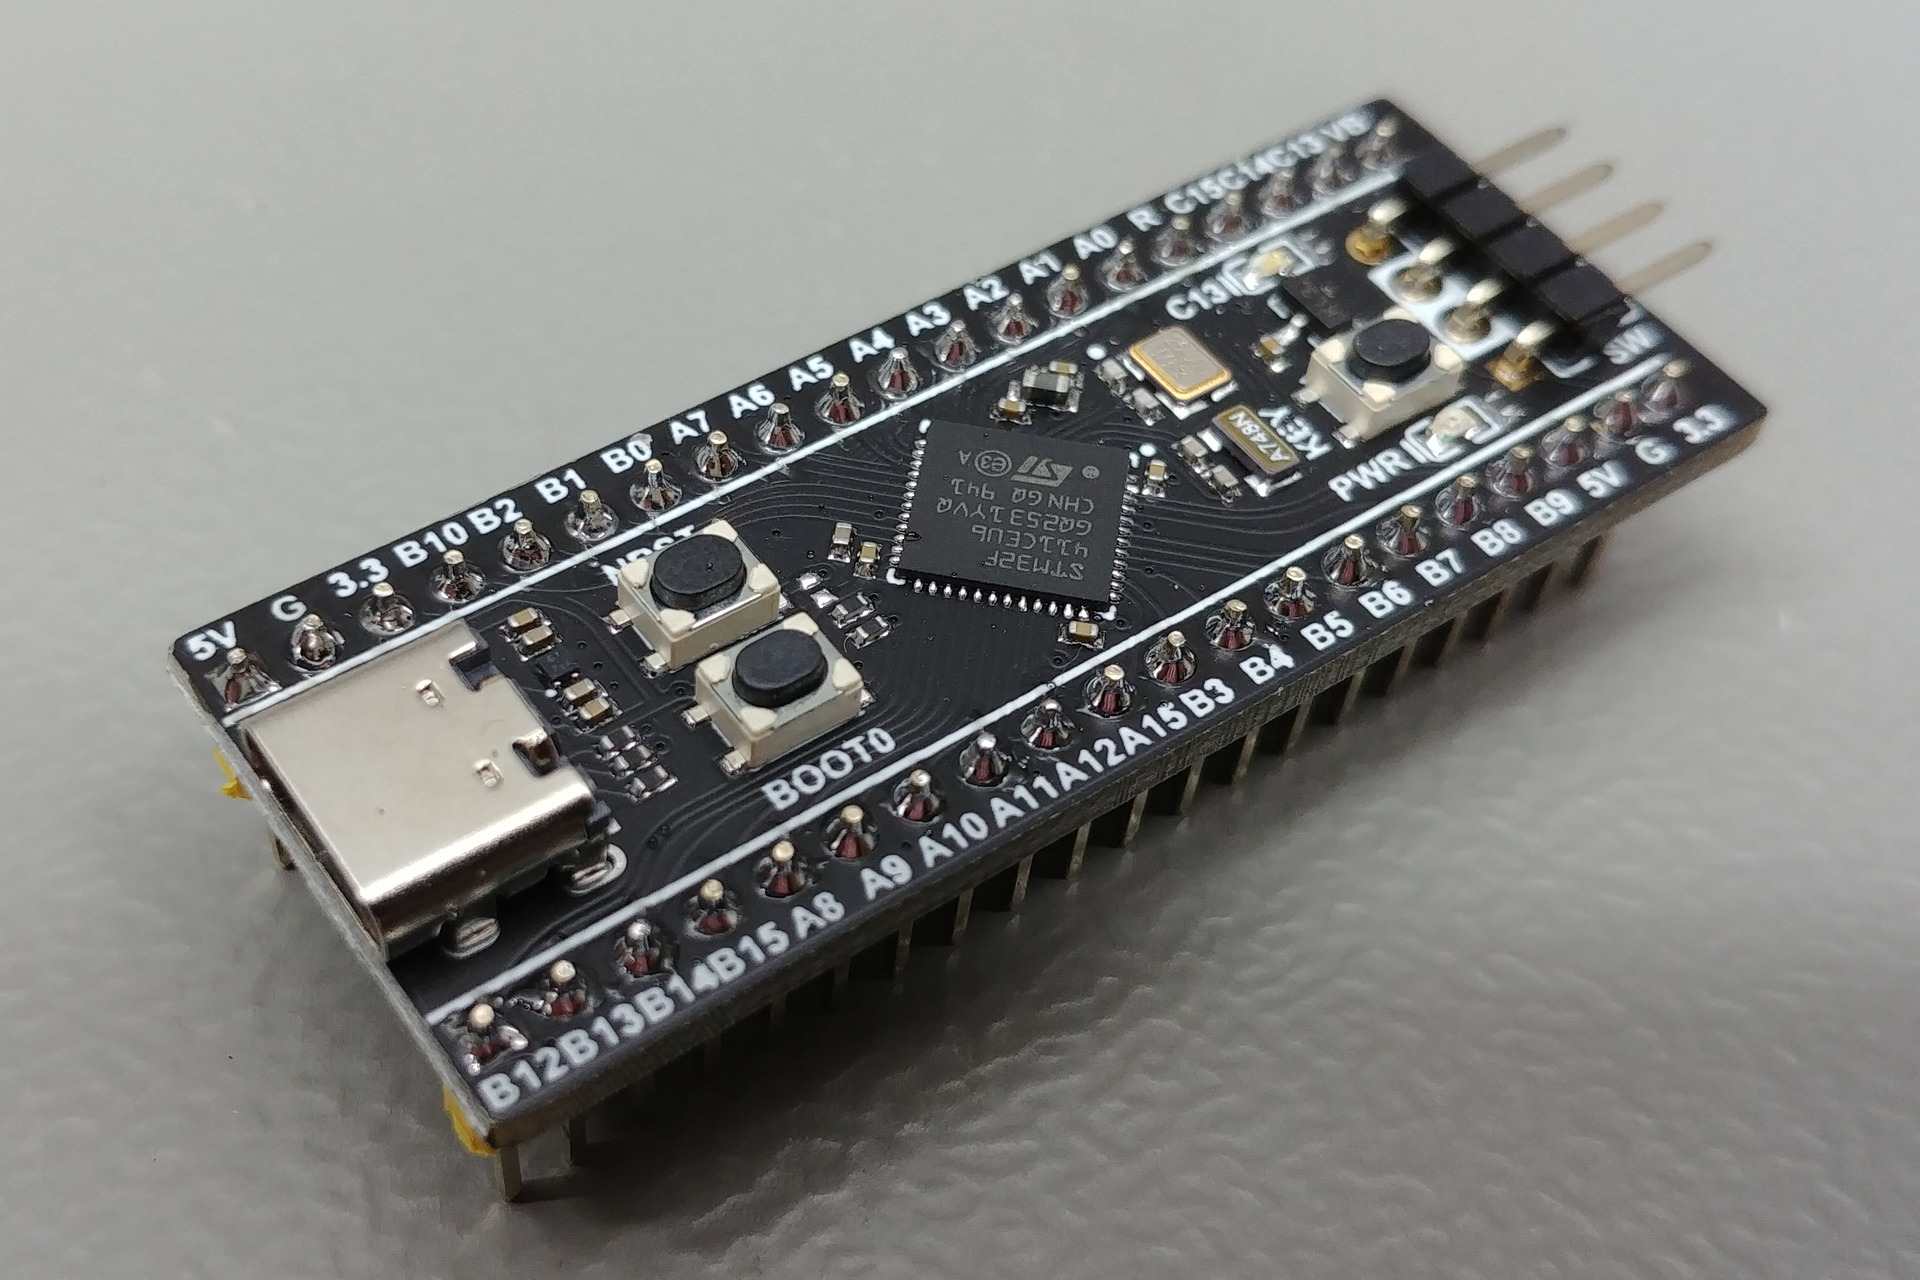
\includegraphics[scale=0.5]{figures/stm32.jpg}
		\end{center}
		\caption{La scheda \texttt{WeAct Black Pill V2.0}.}
		\label{fig:weact_blackpill}
	\end{subfigure}
\end{figure}

\subsection{Schermo}
Lo schermo che abbiamo utilizzato, chiamato \texttt{ILI9341}, è uno schermo LCD
da $2.8''$, con una risoluzione di $320x240$ e controllo individuale dei pixel.
Una particolarità di questo schermo è che offre anche la possibilità di inserire
una scheda microSD al suo interno, che utilizziamo come memoria per i giochi da
utilizzare.
\begin{figure}[h]
	\begin{subfigure}[b]{0.45\textwidth}
		\begin{center}
			\begin{tikzpicture}[x=0.015cm, y=0.015cm, scale=0.5, transform shape]
				\draw   (120, 90) -- (320,90) -- (320,480) -- (120,480) -- cycle ;

\draw  [fill={rgb, 255:red, 255; green, 255; blue, 255 }  ,fill opacity=1 ]  (90,100)  --  (200,100) -- (200,130) --  (90,130) -- cycle;
\draw  [fill={rgb, 255:red, 255; green, 255; blue, 255 }  ,fill opacity=1 ]  (90,130)  --  (200,130) -- (200,160) --  (90,160) -- cycle;
\draw  [fill={rgb, 255:red, 255; green, 255; blue, 255 }  ,fill opacity=1 ]  (90,160)  --  (200,160) -- (200,190) --  (90,190) -- cycle;
\draw  [fill={rgb, 255:red, 255; green, 255; blue, 255 }  ,fill opacity=1 ]  (90,190)  --  (200,190) -- (200,220) --  (90,220) -- cycle;
\draw  [fill={rgb, 255:red, 255; green, 255; blue, 255 }  ,fill opacity=1 ]  (90,220)  --  (200,220) -- (200,250) --  (90,250) -- cycle;
\draw  [fill={rgb, 255:red, 255; green, 255; blue, 255 }  ,fill opacity=1 ]  (90,250)  --  (200,250) -- (200,280) --  (90,280) -- cycle;
\draw  [fill={rgb, 255:red, 255; green, 255; blue, 255 }  ,fill opacity=1 ]  (90,280)  --  (200,280) -- (200,310) --  (90,310) -- cycle;
\draw  [fill={rgb, 255:red, 255; green, 255; blue, 255 }  ,fill opacity=1 ]  (90,310)  --  (200,310) -- (200,340) --  (90,340) -- cycle;
\draw  [fill={rgb, 255:red, 255; green, 255; blue, 255 }  ,fill opacity=1 ]  (90,340)  --  (200,340) -- (200,370) --  (90,370) -- cycle;
\draw  [fill={rgb, 255:red, 255; green, 255; blue, 255 }  ,fill opacity=1 ]  (90,370)  --  (200,370) -- (200,400) --  (90,400) -- cycle;
\draw  [fill={rgb, 255:red, 255; green, 255; blue, 255 }  ,fill opacity=1 ]  (90,400)  --  (200,400) -- (200,430) --  (90,430) -- cycle;
\draw  [fill={rgb, 255:red, 255; green, 255; blue, 255 }  ,fill opacity=1 ]  (90,430)  --  (200,430) -- (200,460) --  (90,460) -- cycle;

\draw  [fill={rgb, 255:red, 255; green, 255; blue, 255 }  ,fill opacity=1 ] (250,100)  --  (380,100) -- (380,130) --  (250,130) -- cycle;
\draw  [fill={rgb, 255:red, 255; green, 255; blue, 255 }  ,fill opacity=1 ] (250,130)  --  (380,130) -- (380,160) --  (250,160) -- cycle;
\draw  [fill={rgb, 255:red, 255; green, 255; blue, 255 }  ,fill opacity=1 ] (250,160)  --  (380,160) -- (380,190) --  (250,190) -- cycle;
\draw  [fill={rgb, 255:red, 255; green, 255; blue, 255 }  ,fill opacity=1 ] (250,190)  --  (380,190) -- (380,220) --  (250,220) -- cycle;
\draw  [fill={rgb, 255:red, 255; green, 255; blue, 255 }  ,fill opacity=1 ] (250,220)  --  (380,220) -- (380,250) --  (250,250) -- cycle;
\draw  [fill={rgb, 255:red, 255; green, 255; blue, 255 }  ,fill opacity=1 ] (250,250)  --  (380,250) -- (380,280) --  (250,280) -- cycle;
\draw  [fill={rgb, 255:red, 255; green, 255; blue, 255 }  ,fill opacity=1 ] (250,280)  --  (380,280) -- (380,310) --  (250,310) -- cycle;
\draw  [fill={rgb, 255:red, 255; green, 255; blue, 255 }  ,fill opacity=1 ] (250,310)  --  (380,310) -- (380,340) --  (250,340) -- cycle;
\draw  [fill={rgb, 255:red, 255; green, 255; blue, 255 }  ,fill opacity=1 ] (250,340)  --  (380,340) -- (380,370) --  (250,370) -- cycle;


\draw (90,460) node [anchor=north west][inner sep=0.75pt]   [align=left] {$\displaystyle SD\_SCK$};
\draw (90,430) node [anchor=north west][inner sep=0.75pt]   [align=left] {$\displaystyle SD\_DO$};
\draw (90,400) node [anchor=north west][inner sep=0.75pt]   [align=left] {$\displaystyle SD\_DI$};
\draw (90,370) node [anchor=north west][inner sep=0.75pt]   [align=left] {$\displaystyle SD\_SS$};
\draw (90,340) node [anchor=north west][inner sep=0.75pt]   [align=left] {$\displaystyle LCD\_D1$};
\draw (90,310) node [anchor=north west][inner sep=0.75pt]   [align=left] {$\displaystyle LCD\_D0$};
\draw (90,280) node [anchor=north west][inner sep=0.75pt]   [align=left] {$\displaystyle LCD\_D7$};
\draw (90,250) node [anchor=north west][inner sep=0.75pt]   [align=left] {$\displaystyle LCD\_D6$};
\draw (90,220) node [anchor=north west][inner sep=0.75pt]   [align=left] {$\displaystyle LCD\_D4$};
\draw (90,190) node [anchor=north west][inner sep=0.75pt]   [align=left] {$\displaystyle LCD\_D5$};
\draw (90,160) node [anchor=north west][inner sep=0.75pt]   [align=left] {$\displaystyle LCD\_D3$};
\draw (90,130) node [anchor=north west][inner sep=0.75pt]   [align=left] {$\displaystyle LCD\_D2$};

\draw (250,370) node [anchor=north west][inner sep=0.75pt]   [align=left] {$\displaystyle 3.3V$};
\draw (250,340) node [anchor=north west][inner sep=0.75pt]   [align=left] {$\displaystyle 5V$};
\draw (250,310) node [anchor=north west][inner sep=0.75pt]   [align=left] {$\displaystyle GND$};
\draw (250,280) node [anchor=north west][inner sep=0.75pt]   [align=left] {$\displaystyle LCD\_RD$};
\draw (250,250) node [anchor=north west][inner sep=0.75pt]   [align=left] {$\displaystyle LCD\_WR$};
\draw (250,220) node [anchor=north west][inner sep=0.75pt]   [align=left] {$\displaystyle LCD\_RS$};
\draw (250,190) node [anchor=north west][inner sep=0.75pt]   [align=left] {$\displaystyle LCD\_CS$};
\draw (250,160) node [anchor=north west][inner sep=0.75pt]   [align=left] {$\displaystyle LCD\_RST$};
\draw (250,130) node [anchor=north west][inner sep=0.75pt]   [align=left] {$\displaystyle F\_CS$};

			\end{tikzpicture}
		\end{center}
		\caption{Pinout dello schermo \texttt{ILI9341}.}
		\label{fig:pinout_ili}

	\end{subfigure}
	\hfill
	\begin{subfigure}[b]{0.45\textwidth}
		\begin{center}
			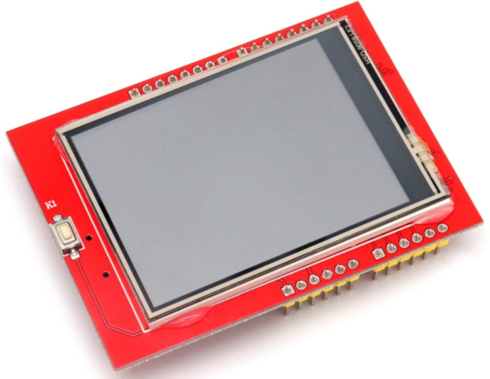
\includegraphics[scale=0.4]{figures/ili.png}
		\end{center}
		\caption{Lo schermo ILI9341.}
		\label{fig:ili9341}
	\end{subfigure}
\end{figure}


\subsection{Gamepad}
L'ultimo componente hardware necessario è la plancia di gioco: per questo
utilizziamo una board costruita appositamente per il form factor del GameBoy
original con $12$ tasti. Ne abbiamo utilizzati solo $8$: frecce direzionali,
\texttt{a}, \texttt{b}, \texttt{select} e \texttt{start}.

\begin{figure}[h]
	\begin{center}
		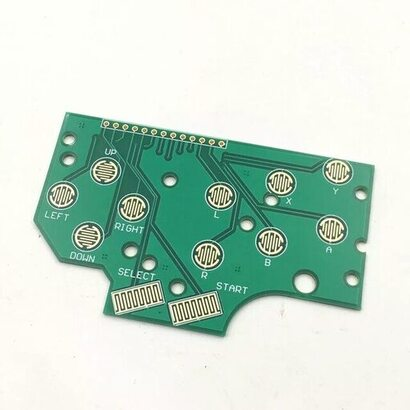
\includegraphics[scale=0.4]{figures/pcb.jpeg}
	\end{center}
	\caption{La PCB GB DMG.}
	\label{fig:pcb}
\end{figure}


\section{Architettura}

\section{Software}
\subsection{Scheda SD}
Fisicamente, la scheda microSD è inserita nello schermo ILI9341, che dispone di
un'apposita porta. La scheda è stata formattata con un filesystem FATFS e
abbiamo adeguato una libreria originariamente per Arduino; questa libreria
permette di leggere

\subsection{Emulatore}
L'emulatore che abbiamo scelto di portare è un emulatore scritto in C per
desktop, chiamato \texttt{peanutGB}. Questo emulatore è distribuito utilizzando
un singolo header C, contenente tutte le funzioni per l'emulazione di un GB,
disponendo per l'utente tutte le funzionalità base per caricare ed eseguire
delle ROM del GB comprese di audio e gestione dei comandi.

\subsubsection{Colori}
Originariamente, il GB disegnava esclusivamente in \textit{grayscale}: ogni
oggetto (sfondo, dialoghi, sprites, transizioni...) è assegnato ad uno dei $4$
\textit{layer} che il GB offre, che viene ulteriormente diviso in $4$
\textit{variables}, come mostrato in \cref{table:gb_colors}.
\begin{table}[h]
	\begin{tabular}{|l|l|llll|}
		\hline
		\textbf{Layer} & \textbf{Description}                                  & \multicolumn{4}{l|}{\textbf{Variables}}                                                          \\ \hline
		\textbf{BG0}   & Sfondo                                                & \multicolumn{1}{l|}{B1}                 & \multicolumn{1}{l|}{B2} & \multicolumn{1}{l|}{B3} & B4 \\ \hline
		\textbf{Win}   & Menu a finestra: stato, pausa, mappa, inventario, HUD & \multicolumn{1}{l|}{W1}                 & \multicolumn{1}{l|}{W2} & \multicolumn{1}{l|}{W3} & W4 \\ \hline
		\textbf{Obj0}  & Sprites principali                                    & \multicolumn{1}{l|}{–}                  & \multicolumn{1}{l|}{S2} & \multicolumn{1}{l|}{S3} & S4 \\ \hline
		\textbf{Obj1}  & Transizioni, sprites secondari                        & \multicolumn{1}{l|}{–}                  & \multicolumn{1}{l|}{P2} & \multicolumn{1}{l|}{P3} & P4 \\ \hline
	\end{tabular}
	\caption{Tabella dei colori per il GB (da
		\cite{GameBoyColors}).}
	\label{table:gb_colors}
\end{table}
L'emulatore \texttt{peanutGB} offre all'utente la possibilità di specificare nel
codice delle \textit{palette} di colori che permettono di mappare layer e
variabili di singoli giochi a colori in formato BGR565.
%\begin{table}[h]
%	\begin{verbatim}
%/* Donkey Kong */
%case 0x19: {
%  const uint16_t palette[3][4] = {
%      {0x7FFF, 0x7E10, 0x48E7, 0x0000}, /* OBJ0 */
%      {0x7FFF, 0x7E10, 0x48E7, 0x0000}, /* OBJ1 */
%      {0x7FFF, 0x7E60, 0x7C00, 0x0000}  /* BG */
%  };
%  memcpy(priv->selected_palette, palette, palette_bytes);
%  break;
%}
%  \end{verbatim}
%\end{table}
\subsubsection{Porting}
%L'emulatore richiede che l'utente definisca alcuni hook
%(descritti in \cref{table:peanutgb_hooks}).
%\begin{table}[h]
%	\begin{verbatim}
%	/**
%	 * Return byte from ROM at given address.
%	 */
%	uint8_t (*gb_rom_read)(struct gb_s*, const uint_fast32_t addr);
%
%	/**
%	 * Return byte from cart RAM at given address.
%	 */
%	uint8_t (*gb_cart_ram_read)(struct gb_s*, const uint_fast32_t addr);
%
%	/**
%	 * Write byte to cart RAM at given address.
%	 */
%	void (*gb_cart_ram_write)(struct gb_s*, const uint_fast32_t addr,
%				  const uint8_t val);
%
%	/**
%	 * Notify front-end of error.
%	 */
%	void (*gb_error)(struct gb_s*, const enum gb_error_e, const uint16_t val);
%      \end{verbatim}
%	\caption{Hook di \texttt{peanutGB} implementati dall'utente.}
%	\label{table:peanutgb_hooks}
%\end{table}
%@TODO

\subsection{Driver ILI}
Per interfacciarsi con lo schermo è stato necessario scrivere un driver
apposito: per questa componente in particolare abbiamo speso buona parte del
tempo necessario per il completamento del progetto. Lo schermo \texttt{ILI9341}
dispone per l'utilizzatore $5$ pin di controllo: \texttt{LCD\_RD},
\texttt{LCD\_WR}, \texttt{LCD\_RS}, \texttt{LCD\_CS}, ed \texttt{LCD\_RST}.
Questi pin vengono utilizzati per modificare lo stato della scheda, come
descritto nella documentazione ufficiale.
\begin{table}[h]
	\begin{verbatim}

  /**
  * Inizializza lo schermo
  */
  int ILI9341_Init(struct ILI9341_t *ili, struct ILI9341_Pin_t D7,
                 struct ILI9341_Pin_t D6, struct ILI9341_Pin_t D5,
                 struct ILI9341_Pin_t D4, struct ILI9341_Pin_t D3,
                 struct ILI9341_Pin_t D2, struct ILI9341_Pin_t D1,
                 struct ILI9341_Pin_t D0, struct ILI9341_Pin_t RST,
                 struct ILI9341_Pin_t CS, struct ILI9341_Pin_t RS,
                 struct ILI9341_Pin_t WR, struct ILI9341_Pin_t RD);

  [...]

  /**
  * Disegna sullo schermo il framebuffer ridimensionato
  */
  void ILI9341_DrawFramebufferScaled(struct ILI9341_t *ili, 
                 uint16_t framebuffer[]);
  \end{verbatim}
	\caption{}
	\label{table:driver_ili}
\end{table}
\subsubsection{Ad alto livello}
Nella \cref{table:driver_ili} mostriamo parte delle funzioni che, ad alto
livello, il driver implementa: ovviamente, \texttt{ILI9341\_Init} è utilizzata
per inizializzare l'unità; \texttt{ILI9341\_DrawFramebufferScaled}, anch'essa
abbastanza auto-esplicativa, è tra le funzioni del driver più utilizzate dal
codice utente. Originariamente il GB mostrava uno schermo $160\times144$: tra le
migliorie che abbiamo implementate vi è anche lo scaling dell'immagine dello
schermo, che è aumentata a $320\times240$.

\subsubsection{Implementazione}
Esaminiamo ora l'implementazione di queste due funzioni. Una struct mantiene lo
stato interno dei collegamenti tra microcontrollore e scheda; tramite le
procedure offerte dal meccanismo GPIO di \texttt{HAL} possiamo impostare lo
stato dei pin dello schermo. La funzione di inizializzazione imposta i pin GPIO
del microcontrollore collegati ai pin di controllo dello schermo come pin di
output.  


\subsection{GUI}
\subsubsection{Font PSF}

\section{Considerazioni finali}
\subsection{Assemblaggio}
Abbiamo speso una buona parte del tempo totale della realizzazione del progetto
a pianificare e tentare vari approcci per l'assemblaggio finale.
\subsection{Potenza}
\subsection{Realizzazione}




\addcontentsline{toc}{section}{References}
\nocite{*}
\printbibliography
\end{document}
